%%%%%%%%%%%%%%%%%%%%%%%%%%%%%%%%%%%%%%%%%
% DOCUMENTACION PASANTIA EN SONDA URUGUAY
% ING. JUAN BRAGA
% MAESTRÍA EN INGENIERÍA ELÉCTRICA, UDELAR
% JUNIO 2016
%%%%%%%%%%%%%%%%%%%%%%%%%%%%%%%%%%%%%%%%%

%----------------------------------------------------------------------------------------
%	PACKAGES AND DOCUMENT CONFIGURATIONS
%----------------------------------------------------------------------------------------

\documentclass{article}

\usepackage[version=3]{mhchem} % Package for chemical equation typesetting
\usepackage{siunitx} % Provides the \SI{}{} and \si{} command for typesetting SI units
\usepackage[spanish]{babel}
\selectlanguage{spanish}
\usepackage[utf8]{inputenc}
\usepackage{graphicx} % Required for the inclusion of images
\usepackage{natbib} % Required to change bibliography style to APA
\usepackage{amsmath} % Required for some math elements 

\setlength\parindent{0pt} % Removes all indentation from paragraphs

\renewcommand{\labelenumi}{\alph{enumi}.} % Make numbering in the enumerate environment by letter rather than number (e.g. section 6)

%\usepackage{times} % Uncomment to use the Times New Roman font

%----------------------------------------------------------------------------------------
%	DOCUMENT INFORMATION
%----------------------------------------------------------------------------------------

\title{\textbf{Desarrollo de módulo de procesamiento de audio en tiempo real con aplicación a seguridad urbana}\\ \textsc{Pasantía Laboral en SONDA Uruguay}\\
\large \textsc{Maestría en Ingeniería Eléctrica} del \textit{Instituto de Ingeniería Eléctrica, Facultad de Ingeniería, Universidad de la República, Uruguay.}}

\author{Ing. Juan \textsc{Braga}}

\date{\today} % Date for the report

\begin{document}

\maketitle % Insert the title, author and date

\begin{center}
\begin{tabular}{l r}
Período: & Diciembre 2015 a Marzo 2016 \\ % Date the experiment was performed
Equipo de SONDA Uruguay: & Msc. Ing. Guillermo Carbajal \\ & Ing. Florencia Lanzaro \\ % Partner names

Docente Responsable: & Msc. Ing. Guillermo Carbajal \\ % Instructor/supervisor
\end{tabular}
\end{center}

% If you wish to include an abstract, uncomment the lines below
% \begin{abstract}
% Abstract text
% \end{abstract}

%----------------------------------------------------------------------------------------
%	SECTION 1
%----------------------------------------------------------------------------------------

\section{Introducción}


El presente informe tiene como objetivo la documentación del desarrollo realizado en SONDA Uruguay en el período de Diciembre 2015 a Marzo 2016, para su aprobación en créditos de la Maestría en Ingeniería Eléctrica de la UdelaR. 

Se detalla sobre un módulo de procesamiento de audio en tiempo real, para funcionamiento embebido en un software de analíticas para seguridad urbana, desarrollado en su totalidad por el equipo de Ingenieros de SONDA Uruguay. 

El software de analíticas actualmente forma parte de la tecnología implantada en el Centro de Monitoreo (CM) del Ministerio del Interior, en el proyecto Ciudad Segura. \cite{Crocco:2016:ASS:2891449.2871183} Tiene como objetivo apoyar la operativa de los visualizadores del CM, alertando automáticamente frente a eventos de interés predefinidos, mediante el procesamiento de Audio y Video en tiempo real.  

\subsection{Sobre SONDA Uruguay}
\label{SONDA Uruguay}

SONDA Uruguay S.A. es fundamentalmente una empresa de servicios y proyectos de integracion de sistemas y provision de plataformas en el campo de las tecnologías de la información. Actualmente SONDA Uruguay S.A. está trabajando en proyectos de I+D en el area de tratamiento de señales, particularmente audio y video. Este equipo de I+D esta conformado por ingenieros de Sistemas y de Eléctrica.


 
%----------------------------------------------------------------------------------------
%	SECTION 2
%----------------------------------------------------------------------------------------

\section{Plataforma de procesamiento}

Los sensores para Seguridad Urbana (en particular las cámaras de video y micrófonos) son diseñados para trabajar en tiempo real, transmitiendo a traves de una red IP los datos adquiridos, a una central donde se realiza el monitoreo y la toma de decisiones. Es en este escenario donde los algoritmos de procesamiento de audio se encuentran embebidos y los tiempos de procesamiento no deben exceder la cadencia de disponibilidad de datos.

La plataforma de procesamiento, se puede dividir en dos grandes bloques: por un lado el de genereración de datos de audio y comunicaciones, y por otro la adquisición desde la red y procesamiento para la toma de decisiones, como se observa en la figura \ref{fig:plataforma_procesamiento}.

De un lado 

El módulo de adquisición hace disponible las muestras de audio, en ventanas de largo configurable según los requerimientos de la algoritmia.

El procesamiento y la toma de decisiones 

\begin{figure}[h]
\begin{center}
\includegraphics[width=0.65\textwidth]{plataforma_procesamiento} 
\caption{Esquema de la plataforma de procesamiento. A la izquierda el bloque de generación y comunicaciones, a la derecha el de adquisición y procesamiento.}
\label{fig:plataforma_procesamiento}
\end{center}
\end{figure}

\section{Analíticas}

Las analíticas son el resultado de la toma de decisiones mediante el procesamiento de señales siendo el trigger de la alarma

\subsection{Umbralizacion en dB}
Tiene como objetivo alertar ante momentos de alto nivel sonoro o ausenci

\subsection{Detección de Sirenas}
For all the following experiments, we extracted Mel-Frequency Cepstral Coefficients (MFCC) from audio slices of \SI{20}{\milli\second} with 50\% frame overlap and hamming windowing. As in  work, we computed 40 Mel bands between 0 and \SI{22050}{\Hz} and kept the first 25 coefficients. 

\begin{figure}[h]
\begin{center}
\includegraphics[width=0.3\textwidth]{deteccion_sirenas} 
\caption{Esquema de la analítica de detección de sirenas. Se observa una primer etapa de substracción de fondo y posterior clasificación en sirena o no.}
\label{fig:deteccion_sirenas}
\end{center}
\end{figure}

\subsubsection{Features}
Se utilizan al igual que en la publicacion \cite{Salamon:UrbanSound:ACMMM:14} los coeficientes MFCC (Mel-Frequency Cepstral Coeficients). 
\subsubsection{Entrenamiento y Clasificación}


%----------------------------------------------------------------------------------------
%	SECTION 3
%----------------------------------------------------------------------------------------

\section{Results}

%\begin{tabular}{ll}
%Mass of magnesium metal & = \SI{8.59}{\gram} - \SI{7.28}{\gram}\\
%& = \SI{1.31}{\gram}\\
%Mass of magnesium oxide & = \SI{9.46}{\gram} - \SI{7.28}{\gram}\\
%& = \SI{2.18}{\gram}\\
%Mass of oxygen & = \SI{2.18}{\gram} - \SI{1.31}{\gram}\\
%& = \SI{0.87}{\gram}
%\end{tabular}

%Because of this reaction, the required ratio is the atomic weight of %magnesium: \SI{16.00}{\gram} of oxygen as experimental mass of Mg: %experimental mass of oxygen or $\frac{x}{1.31}=\frac{16}{0.87}$ from which, %$M_{\ce{Mg}} = 16.00 \times \frac{1.31}{0.87} = 24.1 = \SI{24}{\gram\per%\mole}$ (to two significant figures).

%----------------------------------------------------------------------------------------
%	SECTION 4
%----------------------------------------------------------------------------------------

\section{Conclusions}

The atomic weight of magnesium is concluded to be \SI{24}{\gram\per\mol}, as determined by the stoichiometry of its chemical combination with oxygen. This result is in agreement with the accepted value.



%----------------------------------------------------------------------------------------
%	BIBLIOGRAPHY
%----------------------------------------------------------------------------------------

\bibliographystyle{apalike}
\bibliography{sample}

%----------------------------------------------------------------------------------------


\end{document}